%!TEX root = ../Masterthesis.tex
\chapter{Description of the hand in digital space}
\label{sec:Description_of_hand_in_digital_space}
Tracking of the human hand has always been a challenging problem. In comparison to other larger body parts like the arm or the head, the human hand itself consists of a large variety of smaller components, namely bones and muscles. These components have to be taken into account when trying to replicate the natural motion of the hand in digital space as they all influence the result of the hand motion with their properties.
\section{Physiological structure of the human hand}
\label{sec:Physiological_structure_of_the_human_hand}
Lee and Kuni \citep{LEE.1995} described the human hand as "\textit{an articulated structure with about 30 degrees of freedom [which] changes shape in various ways by its joint movements}"
\begin{figure}[H]
	\centering
	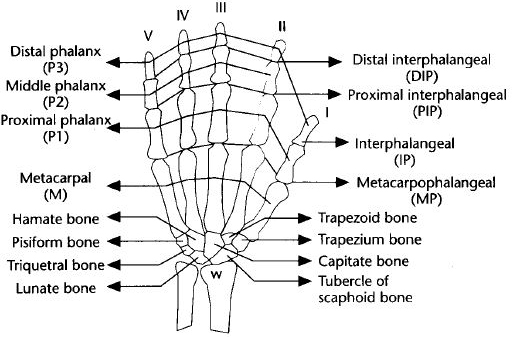
\includegraphics[width=0.8\textwidth]{images/hand.jpg}
	\label{Handstructure} 
	\caption{Bone structure of the left human hand \cite{LEE.1995}}
\end{figure}
All of the hand parts are connected to at least one neighboring part via a \textit{joint}. The \textit{joints} affect the position of the connected part. To describe the movement of the hand parts, we can use the rotation angles of the joints to correlate to a specific position.
To do so, we define a local coordinate system for each of the exiting hand joints. Through these coordinate systems, we achieve a sequence of rotations in the local coordinate systems of the joints. Such a sequence can then be used to describe a specific movement and/or position of a part.
Not all of the joints in the human hand have equal \textit{Degrees of freedom} (DOF's). Their functionality can be classified in the amount of DOF's \cite{KOREIN.1985}:
\begin{flushleft}
\begin{itemize}
\item 1 DOF \\
- A joint movement that can perform a \textbf{flexion} or \textbf{twist} in one direction
\item 2 DOF \\
- A joint movement that can perform \textbf{flexion} in more than one direction (\textbf{directive})
\item 3 DOF\\
- A joint movement that permits simultaneous \textbf{directive} and \textbf{twist} movements.(\textbf{spherical})
\end{itemize}
\end{flushleft}
\begin{figure}[H]
\centering
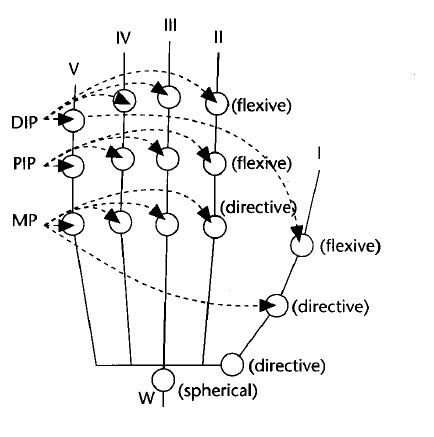
\includegraphics[width=0.6\textwidth]{images/Hand_DOFs.JPG} 
\caption{Types of degrees of freedom for the joints of the human hand}
\label{img:dof_image} 
\end{figure}
When looking at the DOF's displayed in Figure \ref{img:dof_image}, each finger (II-V) sums up to 4 DOF's and the thumb to 5 DOF's. Also considering 6 DOF's for the rotation and position of the whole hand, the sum of all components adds up to 27 DOF's.
\subsection{Constraints in hand motion}
A full usage of all the declared DOF's would lead to a large amount of possible combinations. Since the hand is not only made up of bones but also muscles and the skin, we can impose some constraints \cite{Badler.1987,Pavlovic.1997} to the movement of the joints. Ling, Wu and Huang  \cite{LIN.2000} proposed following classification for the constraints:
\begin{itemize}
\item \textbf{Type I constraints}\\
	- A constraint that limits the range of finger motions based on hand anatomy
	\item \textbf{Type II constraints}\\
	- A constraint that limits the position of the joints during finger movement
	\item \textbf{Type III constraints\\}
	- A constraint that limits position based on natural hand motions
\end{itemize} 
\newpage
The \textbf{Type I} and \textbf{Type II} constraints rely on the physiological and mechanical properties of the human hand. \textbf{Type III} constraints are results of common and natural movements. Therefore these constraints will be differing form person to person. However, these movements are to a certain degree similar for everyone. Accordingly, a broad grouping can be applied. For example, the curling of the fingers at the same time when forming a fist is way more natural than curling each finger by itself. Here the motion of the hand is quite similar between different persons, but the constraints cannot be described in a mathematical form. The examples for the other two constraint types are less complicated.\\\\ For the \textbf{Type I} constraint, there is no doubt that the position of the fingertip is limited by the length of the other finger segments and thereby can only reach as far as the combined length. If you want to touch your hand palm with your fingertip, all joints in the finger have to be bend to achieve this position, which is a constraint example of the \textbf{Type II}. For the mathematical description of \textbf{Type I} and \textbf{Type II} constraints, the following inequalities can be used:\\
\begin{equation}
\begin{split}
0\degree&\leq \Theta _{MP_{flex}} \leq 90\degree\\
0\degree&\leq \Theta _{PIP_{flex}} \leq 110\degree\\
0\degree&\leq \Theta _{DIP_{flex}} \leq 90\degree\\
-15\degree&\leq \Theta _{MP_{abduct/adduct}} \leq 15\degree
\end{split}
\end{equation}
\\For the middle finger, a further specific constraint is applicable, as the middle fingers \textit{Metacarpal} (MP) joint normally does not abduct and adduct much. Therefore an approximation is applicable, resulting in the removal of 1 DOF from the model:\\
\begin{equation}
\Theta _{MP_{abduct/adduct}}=0\degree
\end{equation}
\\The same behavior can be seen in the combination of hand parts labeled \textbf{W} in Figure \ref{img:dof_image} (the connection point between hand and lower arm). This approximation also eliminates 1 DOF on the connected thumb:\\
\begin{equation}
\Theta _{W_{abduct/adduct}}=0\degree
\end{equation}
\\Since the \textit{Distal Interphalangeal} (DIP), \textit{Proximal Interphalangeal}(PIP) and MP joints of our index, middle, ring, and little fingers only have 1 DOF for flexion, we can further assume that their motion is limited to movement in one plane. \\\\
The \textbf{Type II} constraints can be split into \textit{inter-finger} and\textit{ intra-finger} constraints.
Regarding \textit{intra-finger} constraints between the joints of the same finger, human hand anatomy implies certain dependencies. To bend the DIP joints on the specific finger,the corresponding PIP joints of that finger must also be bent.
The approximation for this relation \cite{Rijpkema.1991} can be described as :\\
\begin{equation}
\Theta _{DIP} =\frac{2}{3}\Theta _{PIP}
\end{equation}\\
\\\textit{Inter-finger} constraints can be imposed between joints of adjacent fingers. These constraints describe that the bending of an MP joint in the index finger forces the MP joint in the middle finger to bend as well.\\
When combining the constraints described in the above equations, the initial number 21 DOF's of the human hand can be reduced to 15. Inequalities for these cases, obtained through empiric studies, can be found in \citep{LEE.1995}.\\
\section{Kinematics}
\label{sec:kinematics}
The preceding sections gave an overview of how we can describe a model of the human hand and introduced some limiting constraints. With the model and the constraints, we can now start to build a kinematic system for the animation of the model.\\
Kinematic systems contain so called \textit{kinematic chains}, which consist of a \textit{starting point} or \textit{root}, kinematic elements like \textit{joints}, \textit{links} and an \textit{endpoint}, also called \textit{end-effector}. Applied to the human hand, the whole hand model represents the kinematic system. This system contains several \textit{kinematic chains}, namely the fingers of the hand with the fingertips being the \textit{end-effectors} of each of these chains.
\\Each of these components has it's set of DOF's which can be described mathematically. The established convention for describing this kind of linked systems is the \textit{Denavit-Hartenberg} convention (D-H) \cite{Denavit.1955}. It was originally introduced in order to standardize the coordinate frames for spatial linkages in the field of robotics, but has since then been applied in other fields as well \cite{Spong.2008}. As hand movements starts, the states of the kinematic chains begin to change. Joint angles and end-effector positions are modified until the end position is reached. To represent the new position and angle values of our physical hand with a kinematic system, two major paths for achieving a solution can be taken.
 \subsection{Forward Kinematics}
  \label{sec:Forward Kinematics} 
The \textit{Forward Kinematics} (FK) approach uses the knowledge of the resulting angles and positions after the application of known transformations to the kinematic chain.The resulting new positions of the \textit{joints} and \textit{links} between the \textit{root} and the \textit{end effector} is used to solve the problem of finding the \textit{end-effector's} position.\\
We can denote the existing \textit{end-effectors} relative position to an origin as $ s_{1},...,s_{k}$. The $s_{i}$ position is the result of the combination of all the joint angles in the corresponding kinematic chain. Respectively, we define the target position of the \textit{end-effectors} as $t_{1},...,t_{i}$, with $t_{i}$ being the target position for the \textit{end-effector} $s_{i}$. The required positional change for the \textit{end-effector} can now be described as $e_{i}=t_{i}-s_{i}$. In systems with more than one end-effector, like our hand system, the components can be described by vectors.\\
\begin{equation}
\label{fk components}
\begin{split}
\vec{\textbf{s}}&=(\textbf{s}_{1},...,\textbf{s}_{n})^{T}\\
\vec{\textbf{t}}&=(\textbf{t}_{1},...,\textbf{t}_{n})^{T}\\
\vec{\textbf{e}}&= \vec{\textbf{t}}-\vec{\textbf{s}}\\
\end{split}
\end{equation}
\\As the vector components of $\vec{\textbf{s}}$ are results of the chain joint angles $\theta_{1},...,\theta_{n}$ and therefore are effected by them, we define: \\
\begin{equation}
\label{forward kinematic solution}
\begin{split}
\vec{\textbf{s}_{i}}&=f_{i}(\pmb{\theta})\\
\vec{\textbf{s}}&=f(\pmb{\theta})\\
\end{split}
\end{equation}
\\With $\pmb{\theta}$ being the column vector $\pmb{\theta}=(\theta_{1},...,\theta_{n})^{T}$. The second vector equation displayed in (\ref{forward kinematic solution}) is also called the \textit{Forward Kinematics} (FK) solution.\\
The advantage of an FK solution is that there is always an unique solution to the problem. In consequence, this approach is commonly used in the field of robotics, where the information on the chain elements is easily available.
The tracking of the human hand and all of its chain components is rather complicated when trying to collect all current joint and bone position states. Therefore a solution which takes a known position of the \textit{end-effector} and calculates the parameters for the rest of the chain is more desirable.
\subsection{Inverse kinematics}
\label{sec:inverse kinematics}
\begin{quote}"Inverse Kinematics (IK) is a method for computing the posture via estimating each individual degree of freedom in order to satisfy a given task" \cite{AndreasAristidouandJoanLasenby.2009}\end{quote}
The IK concept already describes it's principle in it's name. It takes the reversed approach in comparison to the FK principle in section \ref{sec:Forward Kinematics}. Instead of knowing the states of the chain elements and calculating the resulting position of the \textit{end-effector}, we take the position of the \textit{end-effector} and try to retrieve the possible states of the other chain elements. \\
\begin{equation}
\label{ik problem formula}
\pmb{\theta}=f^{-1}(\vec{\textbf{s}_{d}})
\end{equation}
\\The result of this equation is the vector $\pmb{\theta}$ for which the values of $\vec{\textbf{s}}$ coincide to the desired configuration $\vec{\textbf{s}_{d}}$. In the case of an optimal result, this configuration would have the same position values as the target positions.\\ The main problem with this method occurs in the calculation of the $f^{-1}$ function, due to it being a highly non linear operator which is not easily invertible.
In contrary to having a unique solution with the FK approach, the IK approach can end at the point of not finding a suitable solution. Figure \ref{IkSolutions} displays three possible outcomes for the IK approach.
\begin{figure}[H]
\centering
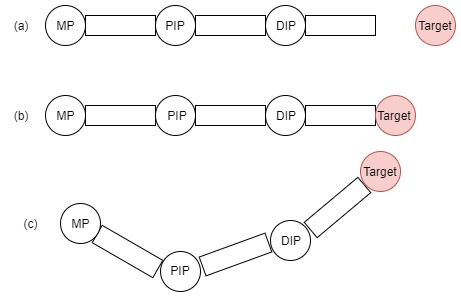
\includegraphics[scale=0.6]{images/Ik_figure.jpg}
\caption{Possible solution for an IK problem of a human finger: (a) The given target position of the end-effector can not be reached. (b) The given target can only be reached by one solution. (c) The target position can be reached with multiple different solutions.}
\label{IkSolutions}
\end{figure}
\subsection{Jacobian-based methods}
\subsubsection{Jacobian inverse}
One common approach to solve the IK problem is the utilization of a \textit{Jacobian} matrix and an iterative calculation process. This matrix contains the partial derivatives of the chain systems relative to the end-effector \textbf{s}. When using the \textit{Jacobian}, a linear approximation  of the IK problem will be applied for solving. The approximation's components model the end-effector's relative movement to changes in transitions of the systems link translations and joint angles. Therefore, the resulting function is dependent on the joint angles $\pmb{\theta}$ values and can be defined as:\\
\begin{equation}
\label{Jacobian definition}
J(\pmb{\theta})_{ij}=\left(\frac{\partial\textbf{s}_{i}}{\partial\theta_{j}}\right)_{ij}
\end{equation}
\\ \textit{i}=1,...,k and \textit{j}= 1,...,n.
Further readings on methods for the calculation of \textit{Jacobian} matrices can be found in \cite{Orin.1984}. Based on Definition (\ref{Jacobian definition}), an entry for the j-th rotational joint would be calculated as follows:\\
\begin{equation}
\label{Jacobian entry calc}
\frac{\partial \textbf{s}_{i}}{\partial \theta_{j}}= \textbf{v}_{j}\times(\textbf{s}_{i}-\textbf{p}_{j})
\end{equation}
\\Here $\textbf{p}_{j}$ is the position of the joint, and $\textbf{v}_{j}$ is the unit vector pointing along the current axis of rotation for the joint.
Taking the derivative of Definition (\ref{forward kinematic solution}) with respect to time gives the basic equation for forward kinematics that describes the velocities of the end-effectors:
\begin{equation}
\label{fk derivate}
\dot{\vec{\pmb{s}}}=\pmb{J}\pmb{(\theta)}\dot{\pmb{\theta}}
\end{equation}
\\ Now having all the values for the angles, the \textit{end-effector} position and the target positions, we can compute the resulting \textit{Jacobian} matrix.
Thereafter we seek an update value $\Delta\pmb{\theta}$ for incrementing the current joint values:\\
\begin{equation}
\label{theta calc}
\pmb{\theta}_{new}=\pmb{\theta}_{curr}+\Delta\pmb{\theta}
\end{equation}
\\The idea here is that the chosen value for $\Delta\pmb{\theta}$ should lead to the resulting $\Delta\pmb{\vec{s}}$ being approximately equal to $\vec{\textbf{e}}$ from (\ref{fk components}). The $\vec{\textbf{e}}$ can be approximated by:\\
\begin{equation}
\label{delta s approx}
\Delta\pmb{\vec{s}}\approx \pmb{J(\theta_{curr})}\Delta\pmb{\theta}
\end{equation}
\\Using this approximation, we can reformulate the FK problem as $\pmb{}\vec{\pmb{e}}=J\Delta\pmb{\theta}$ and therefore our \textit{Inverse Kinematics} problem form \ref{ik problem formula} can be expressed as $ \Delta\pmb{\theta}=J^{-1}\vec{\pmb{e}}$. \\The problem we run into with this solution is the construction of the inverse \textit{Jacobian} matrix. The \textit{Jacobian} matrix \textbf{J} may not be square or invertible. In the case of being invertible, the result may only work inferiorly because of it being nearly singular. Being singular means that no change in joint angle values may achieve the desired end-effector position as an outcome.
\subsubsection{Jacobian transpose}
One approach to calculating the value of $\Delta\pmb{\theta}$ without having to calculate the inverse of \textbf{J} is done by replacing the inverse with the transpose of \textbf{J}.\\
\begin{equation}
\label{delta theta transpose}
\Delta\pmb{\theta}=\alpha \pmb{J}^{T}\vec{\pmb{e}}
\end{equation}
\\Of course the transpose and the inverse of \textbf{J} are not the same thing. When using the theorems displayed in \cite{Orin.1984,Wolovich.1984} we can show that:\\ 
\begin{equation}
\label{transpose show}
\langle JJ^{T}\vec{\pmb{e}},\vec{\pmb{e}}\rangle=\langle J^{T}\vec{\pmb{e}},J^{T}\vec{\pmb{e}}\rangle=\|J^{T}\vec{\pmb{e}}\|\geq 0
\end{equation}
\\Under a sufficiently small $\alpha>0$ the updated angles from \ref{theta calc} will change the end-effector positions by approximately $\alpha JJ^{T}\vec{\pmb{e}}$. They also state that the value of $\alpha$ can be calculated by minimizing the new value of the error vector $\vec{\pmb{e}}$ after each update.\\
\begin{equation}
\label{transpose alpha}
\alpha=\frac{\langle\vec{\pmb{e}},JJ^{T}\vec{\pmb{e}}\rangle}{\langle JJ^{T}\vec{\pmb{e}},JJ^{T}\vec{\pmb{e}}\rangle}
\end{equation}
\subsubsection{Jacobian pseudo inverse}
Instead of calculating the normal inverse of the \textit{Jacoboian}, which can lead to the problems described before, we can use the so called \textit{pseudo-inverse} \cite{Dahmen.2008} for the calculation. The \textit{pseudo inverse} is defined for all matrices \textbf{J}, even ones
which are not square or not of full row rank.\\
\begin{equation}
\label{pseudo inv def}
\Delta\pmb{\theta}=J^{\dagger}\vec{\pmb{e}}
\end{equation}
\\The \textit{pseudo inverse} represents the best possible solution for $ J\Delta\pmb{\theta}=\vec{\pmb{e}}$ in respect to least squares, but does suffer from instability near singularities. It has the property that the matrix $(I − J^{\dagger}J)$ performs a projection onto the null space of \textbf{J} . Therefore, for all vectors $\varphi, J(I −J^{\dagger}J)\varphi = 0$. With this knowledge, $\Delta\pmb{\theta}$ can be calculated by:
\begin{equation}
\Delta\pmb{\theta}=J^{\dagger}\vec{\pmb{e}}+(I-J^{\dagger}J)\varphi
\end{equation}
for any vector $\varphi$ and still obtain a value for $\Delta\theta$ which minimizes the value $ J\Delta\pmb{\theta} −\vec{\pmb{e}}$. The pseudo inverse of \textbf{J} can be derived as follows:\\
\begin{equation}
\begin{split}
\pmb{J}^{\dagger}&=(\pmb{J}^{T}\pmb{J})^{-1}\pmb{J}^{T}\\
\Delta\pmb{\theta}&=(\pmb{J}^{T}\pmb{J})^{-1}\pmb{J}^{T}\vec{\pmb{e}}\\
(\pmb{J}^{T}\pmb{J})\Delta\pmb{\theta}&=\pmb{J}^{T}\vec{\pmb{e}}\\
\end{split}
\end{equation}
\\Using $\vec{\pmb{y}}=\pmb{J}^{T}\vec{\pmb{e}}$, we can now solve the equation $(\pmb{J}^{T}\pmb{J})\Delta\pmb{\theta}=\vec{\pmb{y}}$

\subsection{Singular Value Decomposition}
The usage of a \textit{singular value decomposition} is another method of calculating the \textit{pseudo inverse} of a \textit{Jacobian} matrix. A \textit{singular value decomposition} of \textbf{J} consists of expressing \textbf{J} in the form\\
\begin{equation}
\pmb{J} = \pmb{UDV^{T}}
\end{equation} 
\\For an \textit{m×n} Jacobian matrix, \textbf{U} is\textit{ m×m} and the columns are the \textit{Eigenvectors} of $JJ^{T}$. \textbf{D} is \textit{m×n}, and the entries are zero except along the diagonal where $d_{ii}=\sigma_{i}$ with $\pmb{\sigma_{i}}$ being the singular value and $\sigma 1\geq \sigma 2 \geq ...\geq \sigma m \geq 0$. Singular values are the non-negative square roots of the \textit{Eigenvalues} of $JJ^{T}$ and $ J^{T}J$. \textbf{V} is \textit{n×n} and the columns are the \textit{Eigenvectors} of $J^{T}J$.
The construction of the pseudo inverse is done as follows:\\
\begin{equation}
\pmb{J}^{\dagger} = \pmb{VD^{\dagger}U^{T}}
\end{equation} 
\\The pseudo-inverse of the diagonal matrix \textbf{D} is obtained by replacing each positive diagonal entry with it's reciprocal \cite{Golub.1965}.
\subsection{Damped Least Squares}
 The \textit{Dampened Least Squares} method is applied for inverse kinematics as it avoids the singularity problems that can occur when using the \textit{pseudoinverse}. It further provides a numerical stable method for selecting $\Delta\theta$. First occurences for inverse kinematics can be found in \cite{Wampler.1986,Nakamura.1986}.
Instead of finding the minimum for $\Delta\theta$ as a best solution for the equation displayed in \ref{fk components}, the goal of this method is to find the value that minimizes the following quantity with $\lambda \in \mathbb{R} $ as a dampening factor.\\
\begin{equation}
\parallel J\Delta\pmb{\theta}-\vec{\pmb{e}}\parallel^{2}+\lambda^{2}\parallel\Delta\pmb{\theta}\parallel^{2}
\end{equation}
\\which can be rewritten to the corresponding \\
\begin{equation}
(\pmb{J}^{T}\pmb{J}+\lambda^{2}I)\Delta\pmb{\theta}=\pmb{J}^{T}\vec{\pmb{e}}
\end{equation}
\\and therefore\\
\begin{equation}
\Delta\pmb{\theta}=(\pmb{J}^{T}\pmb{J}+\lambda^{2}I)^{-1}\pmb{J}^{T}\vec{\pmb{e}}
\end{equation}
\\The selection of a correct $\lambda$ value is essential for this method, small values of $\lambda$ give accurate solutions but low robustness to the occurrence of singular and near-singular configurations, while large values of $\lambda$ result in low tracking accuracy even when a feasible and accurate solution would be possible \cite{Chiaverini.1994,AndreasAristidouandJoanLasenby.2009}.

\subsection{Newton Methods}
The family of \textit{Newton methods} is based on a second order Taylor series expansion of the object function \textbf{f(x)}:\\
\begin{equation}
f(x+\sigma)= f(x)+ [\bigtriangledown f(x)]^{T}\sigma + \frac{1}{2}\sigma^{T}H_{f}(x)\sigma
\end{equation}
\\where Hf(x) is the \textit{Hessian matrix}. The downside of this approach is that the calculation of the \textit{Hessian matrix} bares high computational cost for each iteration as a result of its complexity. Like the approximation of the \textit{Jacobian Inverse}, several attempts to lower the computational cost have been made by utilizing an approximation of the \textit{Hessian matrix} based on a function gradient value.
Since the \textit{Newton methods} are posed as a minimization problem, they return smooth motion without erratic discontinuities.
The \textit{Newton methods} also have the advantage that they do not suffer from singularity problems, such as that which occurs when finding the \textit{Jacobian Inverse}.

\subsection{FABRIK Algorithm}
\label{sec:fabrik_algorithm}
A more recent approach in the kinematics field is the \textit{FABRIK} algorithm proposed by Aristidou and Lasenby \cite{Aristidou.2011}. As shown in section \ref{sec:inverse kinematics}, most approaches depend on computational intensive matrix operation like calculating an inverse and may have problems with matrix singularity.\\
\begin{wrapfigure}[43]{r}{7cm}
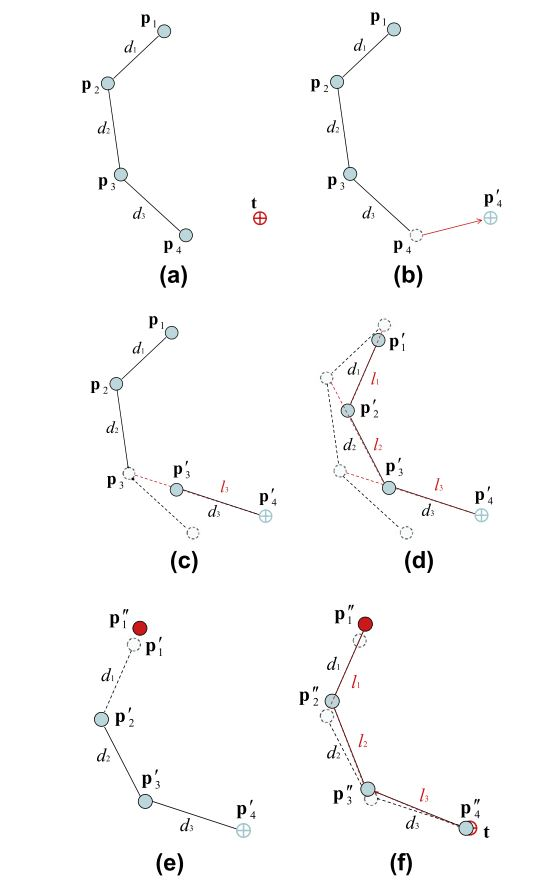
\includegraphics[width=\textwidth/2]{images/FabrikIteration.jpg}
\caption{Forward and backward calculation steps for one iteration of the \textbf{FABRIK}algorithm. (a) Initial position of the system. (b) End effector is moved to target position. (c) Deterimne position of next joint on constructed line. (d) Repeat until root is reached. (e) Move root joint to initial position. (f) Repeat calculation in reverse direction \cite{Aristidou.2011} }
\label{fig:Fabrik_Iteration}
\end{wrapfigure}
The \textit{FABRIK} algorithm does not depend on these matrix operations as is solves for the position of a point on a line to retrieve the new joint positions. This is done in an forward and also inverse solving approach, iterating these steps until the calculated position converges towards the target position from the tracking data.
\\Figure \ref{fig:Fabrik_Iteration} illustrates the steps that are contained in one iteration step.The chain joints are denoted as $\textbf{p}_{\textit{i}}$ with the distance $\textbf{d}_{i}$ being $|\textbf{p}_{\textit{i+1}}-\textbf{p}_{\textit{i}}|$. The \textit{target point} for the \textit{end-effector} is denoted as \textbf{t}.
Step \textbf{(a)} displays the starting point of the iteration. The joint positions are taken from either a previous iteration or from an initial calibration. 
But before calculations can begin, the algorithm has to check whether the intended target point \textbf{t} is reachable for the \textit{end-effector}. This is done by measuring the distance between the root of the \textit{kinematic chain} and the \textit{target point} \textbf{t}. This value is then compared with the sum of the distances $\textbf{d}_{i}$.\\
\begin{equation}
 dist_{t,d_{1}}< \sum_{k=1}^{i}{d_{i}}
\end{equation}
\\If the summed distance is greater, then the target \textbf{t} is within the reach of the system and the calculation can continue, otherwise the calculation has to be aborted and the error has to be manged otherwise.
Assuming this requirement to be met, we can now begin with the first calculation. \\The inverse calculation step is the first step, which is displayed in \textbf{(b)} and \textbf{(c)}. The calculation is started at the end effector, moving to the root of the chain.\newpage
Therefore we assume that the new position $\textbf{p}_{n}^{'}$ with n=4,...,1 is equal to \textbf{t}.\\
\begin{equation}
 \textbf{p}_{n}^{'}=\textbf{t}
\end{equation}
From this new point, we can construct a line that intersects $\textbf{p}_{n}^{'}$ and $\textbf{p}_{n-1}$.\\
\begin{equation}
\begin{split}
A&=\textbf{p}_{n}^{'}\\
B&=\textbf{p}_{n-1}\\
\textbf{l}_{n-1}&=\overline{AB}\\
\end{split}
\end{equation}
\\The resulting position of the new $\textbf{p}_{n-1}^{'}$ point is located on this line with the distance of $\textbf{d}_{n-1}$ from $\textbf{p}_{n}^{'}$ (see \textbf{(c)} ).\\
\begin{equation}
\textbf{p}_{n-1}^{'}= \textbf{p}_{n}^{'}+ \left(\frac{\overline{AB}}{|\overline{AB}|}\cdot\textbf{d}_{n-1}\right)
\end{equation}
\\Consecutively, this is done with the remaining joints until the \textit{root joint} is reached (see \textbf{(d)}).
This finishes the first half of the iteration step. With the calculated positions, we now perform a forward calculation, starting from the root until we reach the \textit{end-effector}. Since the \textit{root} of the system normally does not move from it's initial position, we have to reset the \textit{root joint} to this value before starting to calculate the new positions of the subsequent joints (see\textbf{ (e)}).
\\
Analogous to the procedure in the inverse step, we construct the lines between the points and determine the new position values of the joints. The end result of this step is shown in \textbf{(f)}. At this point, we can decide if the result position of the \textit{end-effector} is appropriate in comparison to the value of \textbf{t}. A simple threshold value for this case could be the position difference between these two points.
\\Since this algorithm does not rely on the heavy-weight matrix operations that the previously described methods incorporate, it converges much faster and in less iterations. Furthermore the incorporation of constraints to the calculation does not interfere with this values and is rather easy.